\chapter{Introduction}
\label{chap:intro}

The autonomous and distributed nature of Internet networks, an intentional consequence of the Internet architecture, can pose difficulty in coordinating networks and their operators to achieve collective action. This observation is visible in the slow progress being made on a number of the challenges that face the Internet today: taking action against spam and malicious behavior, transitioning to a larger Internet address space (IPv6), or adopting more efficient network protocols. These are all cases where the costs and benefits of individual action towards solutions are generally not commensurate, and so no action takes place.

At the same time, the Internet has a relatively strong social network and sense of community amongst its network operators---arguably a historical artifact \cite{Mathew:2010ly}---that can be used to both promote and stigmatize behaviors through social forces such as peer pressure and adherence to norms. This has arguably been successful in achieving economically non-rational behavior on the Internet\footnote{Cases of note include Stanford University returning their /8 block to IANA (``[A]s members of the network community, we need to think about this issue and do the right thing.... It's important for people that have large address space like ours to be good network neighbors.'', \url{http://www.networkworld.com/news/2000/0124ipv4.html}) and more recently, Interop returning their /8 to ARIN \url{https://www.arin.net/announcements/2010/20101020.html}, as well as organizing and participating in the Conficker Working Group \url{http://www.confickerworkinggroup.org/} to combat the Conficker worm. \fbox{more/better examples?}}.
%, and perhaps even cases of collective action. 
While these social forces are probably less strong than they once were, and must now compete with commercial forces stemming from providing Internet service as a business, they are still present as any participant in a network operator community can attest to. 

The purpose of this thesis is to investigate the effectiveness of one case where social forces in the Internet operations community may have played a role in mitigating an Internet collective action problem: the unsustainable growth of the Internet routing table. The objectives of this investigation are twofold. The first is to understand whether the monitoring mechanism that ostensibly spurred the social forces---the CIDR Report---was effective in mitigating this problem. The second is to draw conclusions about approaches to managing the Internet routing table (and possibly inform work on other collective action problems affecting Internet operations and infrastructure) based on lessons learned from analyzing the CIDR Report's efficacy.
%
%These social forces may be useful and perhaps should be considered in designing solutions and building institutions to solve the challenges facing the Internet.

%%%%%%%%%%%%%%%%%%%%%%%%%%%%%%%%%%%%%%%%%%%%%%%%%%%%%%%%%%%%%%%%%%%%%%%%%%%%%%%%
\section{Context and Motivation}

While invisible to most Internet users, interdomain routing is one of the fundamental architectural elements of the Internet. Essentially the defining characteristic of the Internet as a network of networks, interdomain routing enables every network participating in the Internet to locate and exchange traffic with every other Internet-connected network.

In the face of continued growth, the interdomain routing system used by Internet networks faces scalability limits stemming from its design and operation that can limit the ability of network service providers to build and operate networks efficiently. The size and growth rate of the Internet routing table, and specifically the number of prefixes in the table, is one of the major sources of potential scaling issues \cite{rfc4984}. There are a number of causes for this growth, including the addition of new customers and networks in response to increased Internet demand and use, as well as network engineering and the expression of routing policy for existing networks. As shown in Figure \ref{fig:huston_table_plot}, the Internet routing table has grown at a super-linear, sometimes exponential, rate over time \cite{Huston:2001bs}.

\begin{figure}[h]
\begin{center}
    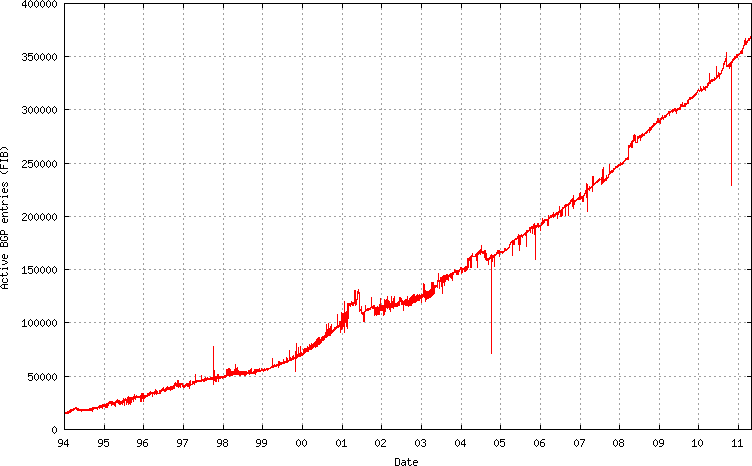
\includegraphics[width=5in]{static_figures/huston_table_plot.png}
    \caption[Growth of the Internet (DFZ) routing table, 1994-present]{Growth of the Internet (DFZ) routing table, 1994-present \cite{6447-table-report}.}
    \label{fig:huston_table_plot}
\end{center}
\end{figure}

% Some claim that engineering efforts -- Moore's law and etc -- make this a non-issue. others claim that the lack of feedback means that this issue lies in wait, and may come back to be problematic

% While currently not a problem, this issue came to the forefront once before in the early 90s. solution was technical change, coupled with social pressure to fix the problem, at a time when there is/was more pain

% we can model the problem as a common-pool resource problem. the internet is the 

Engineering efforts have allowed the capabilities of modern Internet routers to scale more quickly than the growth of the routing table for the most part, allowing the Internet to continue to grow organically without concern. Between evolutionary architectural improvements in succeeding generations of Internet routers \cite{McKeown:2006kx} and the near-guaranteed capacity and performance increases in semiconductors (i.e. Moore's Law), most routers today have capacities that exceed the needs of the Internet routing table. However, these engineering successes have not altered the underlying scaling properties of BGP, the current interdomain routing protocol. While some in the Internet engineering community claim that this is not a pressing concern \cite{Huston:2011ys, Huston:2009dq}, others \cite{Li:2011vn} claim that the lack of any mechanism to control or disincentivize routing table growth means that there is no guarantee that routing table growth will not outpace engineering developments in the future.

Table growth causes engineering trade-offs to be made by router vendors \cite{Li:2011vn, Fall:2009fk} and requires planning and investment consideration by network operators \cite{Zhao:2010fu} at present. While the actual size and growth rate of the routing table has not exceeded the advances provided by Moore's Law, it is exceeding Li's estimate of the constant cost sustainability as shown in Figure \ref{fig:li_router_scalability}. Further, the related challenges of IPv4 exhaustion, which will likely result in advertisement of more, smaller address blocks due to address repurposing and tranfers, and IPv6 adoption, which will drive growth of the IPv6 table\footnote{Which, for a small sample, currently appears exponential: \url{http://bgp.potaroo.net/v6/as6447/}} on dual-stacked routers, may cause routing table growth to accelerate towards unsustainability again. In the long term, unchecked growth could potentially curtail the decentralized, laissez-faire growth and operation that has been a hallmark of the Internet up to this point, or at the very least cause Internet routing to become more expensive than it presently is.

% the theoretical\footnote{or even the more reasonable upper bound of $O(k\,2^{24})$ prefixes based on current RIR and operator policies} upper bound of $O(k\,2^{32})$ prefixes (where $k$ is a constant representing the number peers one connects to) is orders of magnitude beyond the capacity of any current router
\begin{figure}
\begin{center}
    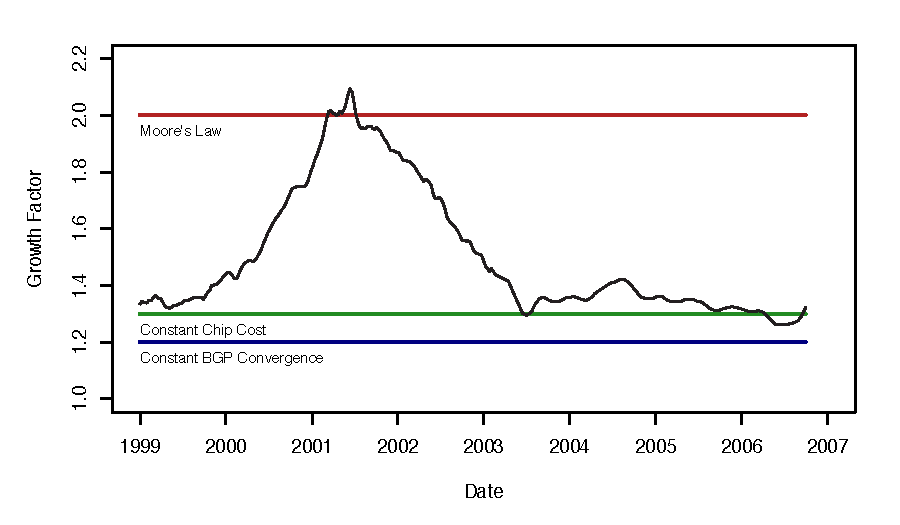
\includegraphics[width=6in]{static_figures/li_relgrowth.pdf}
    \vspace{-2em}\\
    \caption[Normalized growth factors of the Internet routing table relative to Moore's Law]{Normalized growth factors (smoothed over a 2 year window) of the Internet routing table relative to Moore's Law and other desirable engineering objectives, semiconductor chip cost and routing protocol convergence time, from 1999-2007 \cite{Li:2006cr}.}
    \label{fig:li_router_scalability}
\end{center}
\end{figure}

The specter of routing table scaling problems has been encountered once before in the history of the Internet. In the early 1990s, as the Internet was becoming more commercial and moving from a single hierarchical backbone to multiple backbone providers, the Internet routing table began to grow at a rate that would exceed the capabilities of routers available at the time \cite{Huston:2001bs} and in some cases actually did affect the operational behavior of the routers \cite{Li:2011vn}. The solution to this problem was fundamentally a technical one: updating the addressing and routing architecture of the Internet to allow networks to be aggregated, or advertised in larger blocks, thus consuming fewer entries in the routing table. However, the adoption of these technical protocol changes and improvements in operational behavior required to enjoy benefit from these changes was promoted at least in part by social forces within the operator community. 

The mechanism that was used by the Internet operations community to promote more efficient route advertisements was called the CIDR Report. Transmitted weekly to mailing lists associated with major network operator communities, the report contained a section called the ``aggregation report'': an ordered list of the thirty networks that could most reduce the number of entries in the Internet routing table by improving their route announcement behavior. This email report, which was first sent to network operators in approximately 1994, was initially successful in affecting operator behavior. However, at some point it came to be viewed by operators as ineffective\footnote{From correspondence with Martin Hannigan, Patrick Gilmore, Tony Li, and Geoff Huston, as well as \cite{Steenbergen:2010nx}.}. It is interesting that this social mechanism, one that superficially seems to provide only very weak incentives and disincentives, was effective (at least as claimed by a number of network operators and others in the community) in improving on this collective action problem related to technology adoption and efficient route announcement.

%%%%%%%%%%%%%%%%%%%%%%%%%%%%%%%%%%%%%%%%%%%%%%%%%%%%%%%%%%%%%%%%%%%%%%%%%%%%%%%%
\section{The Case of the CIDR Report}

This thesis asks the question of whether the social forces in the Internet operations community are capable of inducing collective action. This question is asked in the context of one specific case: the CIDR Report and its ability to control the growth of the Internet routing table. The working hypothesis for this question is that appearing on the CIDR Report did not significantly affect operator behavior. This position is based on discussions with network operators and observation of the continually-increasing number of prefixes in the routing table as shown in Figure \ref{fig:huston_table_plot}.

The case of the CIDR Report and routing table growth is of interest and particularly well suited for this analysis for a number of reasons. First, this case runs over a long period of time, starting in 1997, so there is a good opportunity to observe community and individual operator behavior. This long duration is backed by a large amount of publicly available data to support the analysis of the report, including the CIDR Report emails themselves as well as archived views of the Internet routing table. The CIDR Report is naturally suited to allow for a quasi-experiment in that only part of the population is ``treated'' by the CIDR Report, while the rest of the population is available for use as a control. Finally, the CIDR Report was and is a well-known and well-publicized phenomenon within the operator community, and was created with the intent of educating and also socially pressuring operators, and so should be a suitable case for assessing the effects of social forces within the Internet operator community.

Other potential cases involving the social forces within the operator community, such as the backchannel communications mentioned in \cite{Mathew:2010ly}, are difficult to study as there is typically a lack of data, a lack of publicity of the events that occur that motivate social pressure, and the events of potential interest for analysis are somewhat ad-hoc and randomly distributed (e.g. the YouTube hijacking \cite{Brown:2008hc}).

% sentence here????

As with any study of a single case, it is generally not possible to make generalizations about the broader question based the results of the study. Thus, while this thesis is motivated by the potential use of social forces to solve collective action problems of Internet operations, conclusions drawn from my study of the CIDR Report may not be useful in providing insights for other cases. However, any interesting insights about this case may be starting points for further study and exploration in other cases.

%%%%%%%%%%%%%%%%%%%%%%%%%%%%%%%%%%%%%%%%%%%%%%%%%%%%%%%%%%%%%%%%%%%%%%%%%%%%%%%%
\section{The Routing Table as a Common Pool Resource}

The unconstrained growth of the Internet routing table is often considered a commons problem: individuals derive private benefit from adding entries to the table, but each entry incurs a public cost---a negative externality---for all others that participate in the Internet routing system. The public cost is not necessarily trivial either, with one network operator roughly estimating the marginal cost of a BGP prefix at \$6000-\$8000 per year \cite{Herrin:2008qa} and a researcher estimating the same figure at \$77,000 over the lifetime of the router \cite{Clayton:2010bh}. This cost is not borne by any one network, but is the estimated cost of the fraction of router resources consumed by one route across all BGP-speaking routers with a full (DFZ) routing table worldwide.

Discussions of the problem \cite{Huston:2001bs,Clayton:2010bh,Bellovin:2001qf} often invoke Hardin's \cite{Hardin:1968uq} notion of the tragedy of the commons---that individually rational actors will attempt to maximize consumption of a resource because they privately enjoy the full benefit of this consumption but share the cost of its reduced capacity, making all actors worse off. Common solutions advocated for such problems are the establishment of a central regulator or private property rights. However, the Internet routing table and interdomain routing lacks both such features and has not yet been reduced to tragedy. This is arguably a result, at least in part, of the ``property rights'' and governance regime of the interdomain routing system. By understanding these characteristics, it may be helpful in understanding how and why the CIDR Report had effect while also offering insights into other approaches to enable more effective management of the routing table.

In contrast to the broad notion of a ``commons problem'', Ostrom \cite{Ostrom:1990fv} presents the more nuanced concept of common pool resources (CPR) and CPR management problems. Her work has mostly focused on the management of natural resources such as fisheries, forests, and aquifers, but the general elements of the framework are applicable to other cases as well. In Ostrom's model of common pool resources, the \emph{resource system} (such as a fishery) is considered separately from the subtractable \emph{resource units} (in this example, fish) that can be extracted from the resource. The resource system produces some number of units that can be extracted sustainably, and beyond that point extraction causes harm to the system itself. Actors that extract resource units are referred to as \emph{appropriators} (fishers), and actors that take efforts to improve or sustain the resource (such as farming and stocking bodies of water with fish) are \emph{producers}. If the resource system is not naturally occurring, then it must be created or organized by \emph{providers}. In all cases, the essential defining qualities of a CPR are that it is difficult to exclude others from using the resources (there are no private property rights), and that the resource is rivalrous (the use of the resource by one actor precludes its use by another).

The CPR framework can also be mapped relatively cleanly to the case of the Internet routing table. The Internet's interdomain routing system is a CPR resource system provided collectively by every network that maintains a router with a full table of BGP routes. 
%Operators of more popular or higher-traffic networks ostensibly must buy more equipment and thus pay a higher cost for their part of the system in order to meet demand, but in the case of content provider or ISPs this is often compensated for by payments (though based on traffic, not on routing table prefixes). 
There is not a single global routing table---each provider maintains its own version of the global routing table. However, the value in the routing table is its consistency and uniqueness across all Internet participants in order to allow global reachability. It is technically feasible for one network to exclude others' routes from the routing table, but the value of the interdomain routing system is in global reachability, and so it is difficult to exclude routes without potentially reducing the utility of the network's connectivity to the Internet. 

Routing table capacity (``slots'' or routes) are the resource units of the routing table CPR. Routing table entries are not intrinsically valuable in that they cannot be ``extracted'' and used elsewhere. However, they are valuable in that they permit interconnection and reachability to the rest of the Internet. It is necessary for each network connected to the Internet to occupy at least one slot in order to make a network available to the Internet, and its often desirable to consume multiple slots for engineering or routing policy reasons. Thus, networks must appropriate routing table slots to participate in the Internet. These slots are rivalrous in that each router has a limited capacity and slots used by one network's route announcements cannot be used by another. As a public system with rival resource units, the interdomain routing system has the hallmark characteristics of a CPR.

Mueller \cite{Mueller:2010bh} supports a similar view of the routing table as a CPR, arguing that while IP addresses and address blocks could be handled as private property, they are managed as common pool goods to protect the routing table. He suggests that RIR address allocation policy is used to conserve routing table slots by enforcing route aggregation and preventing IP address block fragmentation that might result from reselling address blocks.

Under the CPR model, Ostrom's appropriators are rational individuals who make decisions based on four inputs: the costs of a particular strategy, the benefits of a particular strategy, their internal discount rate (the relative perceived value of future benefits versus present benefits), and their internal norms. What is notable about the appropriators in some CPR cases is that they have learned about the limits of their resource system through trial and error and, unlike the fictional rational grazers of Hardin's commons, communicate with other appropriators to establish institutions that govern the appropriation of units in an effort to ensure sustainability of the resource system. Such institutions work to affect the decision-making algorithm of appropriators by increasing the costs of a particular strategy through sanctions, or establishing norms that are then internalized by the appropriator, which in turn affect perceptions of costs and benefits.

% trust, small communities, etc.

CPR governance institutions---which usually include commitment to acceptable behavior as well as mutual monitoring and sanction mechanisms to limit opportunistic behavior---are not guaranteed to exist when a CPR is provided, or or to be effective even when they do exist. However, there is evidence that some form of community-based governance institution has had an effect on the routing table, such as Huston's observation of decreases in routing table size following IETF meetings in the mid-1990s \cite{Huston:2001bs,Clayton:2010bh}. In the case of the routing table, there are no explicitly obvious sanction mechanisms beyond shame, criticism, and peer pressure of the network operator community, which may affect the reputation of network providers and the individuals operating their networks. Internalization of community norms of cooperation and collegiality \cite{Abbate:2000ve} likely also contributed in the case of the routing table.

In this context, the CIDR Report can be considered a mutual monitoring mechanism that provided information about adherence to norms for the loosely-defined, norm-based governance institution. It was not created or mutually agreed upon by the community, but instead offered to the community by a few individuals as part of the CIDR deployment effort, though its conclusions could be verified by anyone with access to a router. The information provided by the CIDR Report was embraced by some network operators as a basis for invoking sanctions of shame and peer pressure that are sometimes visible on the NANOG mailing list \cite{NANOG}, and it also affected operator behavior via internal norms\footnote{In \cite{Li:2011vn}, Li notes that Cisco clients sought advice and help to improve their aggregation after appearing on the CIDR Report.}. However, as many operators have observed or conceded, the CIDR Report appears to be less effective than it once was.

If we accept the view of the interdomain routing system and Internet routing table as a CPR, and the CIDR Report as part of the loosely-defined governance institution for the routing table, it may be helpful to apply Ostrom's frameworks and analysis to the problem of managing the routing table. The framework may be instructive in seeking to understand the causes of variation in behavior change induced by the CIDR Report over time that have caused operators to perceive the report as less effective. Further, it may provide insights about other approaches to managing the Internet routing table.

%%%%%%%%%%%%%%%%%%%%%%%%%%%%%%%%%%%%%%%%%%%%%%%%%%%%%%%%%%%%%%%%%%%%%%%%%%%%%%%%
\section{Contributions of this thesis}

This thesis makes a number of contributions to the space of Internet routing table analysis, including:
\begin{itemize}
\item{A history of the CIDR Report, as presented in Chapter \ref{chap:background}.}
\item{A well-documented, open-source implementation of the CIDR Report aggregation report algorithm that utilizes multiple vantage points, as described in Chapter \ref{chap:method} and Appendix \ref{chap:opensource}.}
\item{An analysis of the characteristics of the CIDR Report, including the distribution of networks that appear on it, etc., as presented in Chapter \ref{chap:analysis}.}
\item{An analysis of the effects of appearing on the CIDR Report on the route announcement behavior of individual networks, also presented in Chapter \ref{chap:analysis}.}
%\item{An analysis of network deaggregation behavior on a per-AS basis, unlike other table-wide analyses.}
\item{Consideration of the CIDR Report as CPR governance institution for the Internet routing table.}
\end{itemize}

%%%%%%%%%%%%%%%%%%%%%%%%%%%%%%%%%%%%%%%%%%%%%%%%%%%%%%%%%%%%%%%%%%%%%%%%%%%%%%%%
\section{Roadmap for remaining chapters}

The remainder of this thesis proceeds as follows. Chapter 2 presents a broad overview of relevant background information in this space, both for the reader who may be unfamiliar with interdomain routing on the Internet, as well as those who wish to understand some of the finer points that motivate Internet operations and routing table growth. This chapter also contains an overview CIDR Report and a brief history of the events that motivated its creation and evolution over time. 

Chapter 3 describes the analytical approach taken to determine whether the CIDR Report was effective. It begins by describing the data sources that were used to conduct the analysis and the preprocessing steps taken against that data. Next, the algorithms and methods used to generate the CIDR Report and its aggregation report are described. Finally, the approach taken to analyze AS behavior over time is presented and described. 

Chapter 4 presents and discusses the results of this analysis: it considers both the overall characteristics of the CIDR Report and the networks that appear on it, as well as a specific analysis of the behavior of networks that appear on the CIDR Report. 

Following the presentation of these analytical results, Chapter 5 discusses a number of reasons for why the efficacy of the CIDR Report may have changed over time by considering the routing table growth situation through the lens of Ostrom's common pool resource framework.

Chapter 6 presents a review of related work from the literature and other sources on measurement and analysis of the growth of the Internet routing table, solutions to the scalability challenges facing interdomain routing, and characteristics of the Internet operations community.

Finally, Chapter 7 offer a concluding discussion and recommendations regarding the management of the Internet routing table, as well as how these observations might be used to design institutions to solve other problems facing the Internet.